%%%%%%%%%%%%%%%%%%%%%%%%%%%%%%%%%%%%%%%%%
% Classicthesis Typographic Thesis
% LaTeX Template
% Version 1.1 (4/8/12)
%
% This template has been downloaded from:
% http://www.LaTeXTemplates.com
%
% Original author:
% André Miede (http://www.miede.de)
%
% License:
% CC BY-NC-SA 3.0 (http://creativecommons.org/licenses/by-nc-sa/3.0/)
%
% General Tips:
% 1) Make sure to edit the classicthesis-config.file
% 2) New enumeration (A., B., C., etc in small caps): \begin{aenumerate} \end{aenumerate}
% 3) For margin notes: \marginpar or \graffito{}
% 4) Do not use bold fonts in this style, it is designed around them
% 5) Use tables as in the examples
% 6) See classicthesis-preamble.sty for useful commands
%
%%%%%%%%%%%%%%%%%%%%%%%%%%%%%%%%%%%%%%%%%

%----------------------------------------------------------------------------------------
%	PACKAGES AND OTHER DOCUMENT CONFIGURATIONS
%----------------------------------------------------------------------------------------

\documentclass[
		twoside,openright,titlepage,numbers=noenddot,headinclude,%1headlines,
                footinclude=true,cleardoublepage=empty,
                BCOR=5mm,paper=a4,fontsize=11pt, % Binding correction, paper type and font size
                english, % Languages
                ]{scrreprt} 
                
% Includes the file which contains all the document configurations and packages - make sure to edit this file
%%%%%%%%%%%%%%%%%%%%%%%%%%%%%%%%%%%%%%%%%
% Thesis Configuration File
%
% The main lines to change in this file are in the DOCUMENT VARIABLES
% section, the rest of the file is for advanced configuration.
%
%%%%%%%%%%%%%%%%%%%%%%%%%%%%%%%%%%%%%%%%%

%----------------------------------------------------------------------------------------
%	DOCUMENT VARIABLES
%	Fill in the lines below to enter your information into the thesis template
%	Each of the commands can be cited anywhere in the thesis
%----------------------------------------------------------------------------------------

% Remove drafting to get rid of the '[ Date - classicthesis version 4.0 ]' text at the bottom of every page
\PassOptionsToPackage{eulerchapternumbers,listings,pdfspacing,subfig,beramono,eulermath,parts,dottedtoc,tocaligned}{classicthesis}
% Available options: drafting parts nochapters linedheaders eulerchapternumbers beramono eulermath pdfspacing minionprospacing tocaligned dottedtoc manychapters listings floatperchapter subfig
% Adding 'dottedtoc' will make page numbers in the table of contents flushed right with dots leading to them

\newcommand{\myTitle}{Endpoint Compliance Monitoring based on Software Identification Tags\xspace}
\newcommand{\mySubtitle}{TODO subtitle\xspace}
\newcommand{\myThesis}{Bachelorarbeit\xspace}
\newcommand{\myName}{Christian F{\"a}ssler, Danilo Bargen Jonas Furrer\xspace}
\newcommand{\myProf}{Prof. Dr. Andreas Steffen\xspace}
\newcommand{\myFaculty}{ITA Institute for Internet Technologies and Applications\xspace}
\newcommand{\myDepartment}{Abteilung Informatik\xspace}
\newcommand{\myUni}{HSR Hochschule f{\"u}r Technik Rapperswil\xspace}
\newcommand{\myLocation}{Rapperswil\xspace}
\newcommand{\myTime}{Fr{\"u}hling 2014\xspace}
\newcommand{\myVersion}{version 1.0\xspace}
\newcommand{\myLicense}{CC BY-SA 3.0 Unported\xspace}
\newcommand{\myKeywords}{SWID, TNC, StrongSwan, IPsec, Compliance Monitoring}

%----------------------------------------------------------------------------------------
%	USEFUL COMMANDS
%----------------------------------------------------------------------------------------

\newcounter{dummy} % Necessary for correct hyperlinks (to index, bib, etc.)
\providecommand{\mLyX}{L\kern-.1667em\lower.25em\hbox{Y}\kern-.125emX\@}

%----------------------------------------------------------------------------------------
%	PACKAGES
%----------------------------------------------------------------------------------------

\usepackage{lipsum} % Used for inserting dummy 'Lorem ipsum' text into the template

%------------------------------------------------
 
\PassOptionsToPackage{utf8}{inputenc}
\usepackage{inputenc}
 
%------------------------------------------------

\PassOptionsToPackage{american}{babel}
\usepackage{babel}

%------------------------------------------------			

\PassOptionsToPackage{square,numbers}{natbib}
\usepackage{natbib}
 
%------------------------------------------------

\PassOptionsToPackage{fleqn}{amsmath} % Math environments and more by the AMS 
\usepackage{amsmath}
 
%------------------------------------------------

\PassOptionsToPackage{T1}{fontenc}
\usepackage{fontenc}

%------------------------------------------------

\usepackage{xspace} % To get the spacing after macros right

%------------------------------------------------

\usepackage{mparhack} % To get marginpar right

%------------------------------------------------

\usepackage{fixltx2e} % Fixes some LaTeX stuff 

%------------------------------------------------

\PassOptionsToPackage{smaller}{acronym} % Include printonlyused in the first bracket to only show acronyms used in the text
\usepackage{acronym} % nice macros for handling all acronyms in the thesis

%------------------------------------------------

%\renewcommand*{\acsfont}[1]{\textssc{#1}} % For MinionPro
\renewcommand{\bflabel}[1]{{#1}\hfill} % Fix the list of acronyms

%------------------------------------------------

\PassOptionsToPackage{pdftex}{graphicx}
\usepackage{graphicx} 
\usepackage{subfig}

%------------------------------------------------

\usepackage{pgf} 
\usepackage{tikz} 
\usepackage{tikz-qtree}
\usetikzlibrary{}

%------------------------------------------------

\usepackage{wrapfig}

%------------------------------------------------

\usepackage{siunitx}


%----------------------------------------------------------------------------------------
%	FLOATS: TABLES, FIGURES AND CAPTIONS SETUP
%----------------------------------------------------------------------------------------

\usepackage{tabularx} % Better tables
\setlength{\extrarowheight}{3pt} % Increase table row height
\newcommand{\tableheadline}[1]{\multicolumn{1}{c}{\spacedlowsmallcaps{#1}}}
\newcommand{\myfloatalign}{\centering} % To be used with each float for alignment
\usepackage{caption}
\captionsetup{format=hang,font=small}
\usepackage{subfig}  

%----------------------------------------------------------------------------------------
%	CODE LISTINGS SETUP
%----------------------------------------------------------------------------------------

\usepackage{minted} % Syntax highlighting                                                                                                                                                                                                      
\usemintedstyle{tango}
\definecolor{tango-bg}{HTML}{F8F8F8}

\newminted{python}{bgcolor=tango-bg,frame=lines,framesep=2mm,samepage=true,fontsize=\footnotesize}

%\usepackage{listings} 
%\lstset{emph={trueIndex,root},emphstyle=\color{BlueViolet}}%\underbar} % for special keywords
%\lstset{language=Python, % Specify the language for listings here
%keywordstyle=\color{RoyalBlue}, % Add \bfseries for bold
%basicstyle=\small\ttfamily, % Makes listings a smaller font size and a different font
%%identifierstyle=\color{NavyBlue}, % Color of text inside brackets
%commentstyle=\color{Green}\ttfamily, % Color of comments
%stringstyle=\rmfamily, % Font type to use for strings
%numbers=left, % Change left to none to remove line numbers
%numberstyle=\scriptsize, % Font size of the line numbers
%stepnumber=5, % Increment of line numbers
%numbersep=8pt, % Distance of line numbers from code listing
%showstringspaces=false, % Sets whether spaces in strings should appear underlined
%breaklines=true, % Force the code to stay in the confines of the listing box
%%frameround=ftff, % Uncomment for rounded frame
%frame=single, % Frame border - none/leftline/topline/bottomline/lines/single/shadowbox/L
%belowcaptionskip=.75\baselineskip % Space after the "Listing #: Desciption" text and the listing box
%}

%----------------------------------------------------------------------------------------
%	HYPERREFERENCES
%----------------------------------------------------------------------------------------

\PassOptionsToPackage{pdftex,hyperfootnotes=false,pdfpagelabels}{hyperref}
\usepackage{hyperref}  % backref linktocpage pagebackref
\pdfcompresslevel=9
\pdfadjustspacing=1

\hypersetup{
% Uncomment the line below to remove all links (to references, figures, tables, etc)
%draft, 
colorlinks=true, linktocpage=true, pdfstartpage=1, pdfstartview=FitV,
% Uncomment the line below if you want to have black links (e.g. for printing black and white)
%colorlinks=false, linktocpage=false, pdfborder={0 0 0}, pdfstartpage=1, pdfstartview=FitV, 
breaklinks=true, pdfpagemode=UseNone, pageanchor=true, pdfpagemode=UseOutlines,
plainpages=false, bookmarksnumbered, bookmarksopen=true, bookmarksopenlevel=1,
hypertexnames=true, pdfhighlight=/O, urlcolor=webbrown, linkcolor=RoyalBlue, citecolor=webgreen,
%------------------------------------------------
% PDF file meta-information
pdftitle={\myTitle},
pdfauthor={\textcopyright\ \myName, \myUni, \myFaculty},
pdfsubject={\mySubtitle},
pdfkeywords={\myKeywords},
pdfcreator={pdfLaTeX},
pdfproducer={LaTeX with hyperref and classicthesis}
%------------------------------------------------
}   

%----------------------------------------------------------------------------------------
%	BACKREFERENCES
%----------------------------------------------------------------------------------------

\usepackage{ifthen} % Allows the user of the \ifthenelse command
\newboolean{enable-backrefs} % Variable to enable backrefs in the bibliography
\setboolean{enable-backrefs}{false} % Variable value: true or false

\newcommand{\backrefnotcitedstring}{\relax} % (Not cited.)
\newcommand{\backrefcitedsinglestring}[1]{(Cited on page~#1.)}
\newcommand{\backrefcitedmultistring}[1]{(Cited on pages~#1.)}
\ifthenelse{\boolean{enable-backrefs}} % If backrefs were enabled
{
\PassOptionsToPackage{hyperpageref}{backref}
\usepackage{backref} % to be loaded after hyperref package 
\renewcommand{\backreftwosep}{ and~} % separate 2 pages
\renewcommand{\backreflastsep}{, and~} % separate last of longer list
\renewcommand*{\backref}[1]{}  % disable standard
\renewcommand*{\backrefalt}[4]{% detailed backref
\ifcase #1 
\backrefnotcitedstring
\or
\backrefcitedsinglestring{#2}
\else
\backrefcitedmultistring{#2}
\fi}
}{\relax} 

%----------------------------------------------------------------------------------------
%	AUTOREFERENCES SETUP
%	Redefines how references in text are prefaced for different 
%	languages (e.g. "Section 1.2" or "section 1.2")
%----------------------------------------------------------------------------------------

\makeatletter
\@ifpackageloaded{babel}
{
\addto\extrasamerican{
\renewcommand*{\figureautorefname}{Figure}
\renewcommand*{\tableautorefname}{Table}
\renewcommand*{\partautorefname}{Part}
\renewcommand*{\chapterautorefname}{Chapter}
\renewcommand*{\sectionautorefname}{Section}
\renewcommand*{\subsectionautorefname}{Section}
\renewcommand*{\subsubsectionautorefname}{Section}
}
\addto\extrasngerman{
\renewcommand*{\paragraphautorefname}{Absatz}
\renewcommand*{\subparagraphautorefname}{Unterabsatz}
\renewcommand*{\footnoteautorefname}{Fu\"snote}
\renewcommand*{\FancyVerbLineautorefname}{Zeile}
\renewcommand*{\theoremautorefname}{Theorem}
\renewcommand*{\appendixautorefname}{Anhang}
\renewcommand*{\equationautorefname}{Gleichung}
\renewcommand*{\itemautorefname}{Punkt}
}
\providecommand{\subfigureautorefname}{\figureautorefname} % Fix to getting autorefs for subfigures right
}{\relax}
\makeatother

%----------------------------------------------------------------------------------------

\usepackage{classicthesis} 

%----------------------------------------------------------------------------------------
%	CHANGING TEXT AREA 
%----------------------------------------------------------------------------------------

%\linespread{1.05} % a bit more for Palatino
%\areaset[current]{312pt}{761pt} % 686 (factor 2.2) + 33 head + 42 head \the\footskip
%\setlength{\marginparwidth}{7em}%
%\setlength{\marginparsep}{2em}%

%----------------------------------------------------------------------------------------
%	USING DIFFERENT FONTS
%----------------------------------------------------------------------------------------

%\usepackage[oldstylenums]{kpfonts} % oldstyle notextcomp
%\usepackage[osf]{libertine}
%\usepackage{hfoldsty} % Computer Modern with osf
%\usepackage[light,condensed,math]{iwona}
%\renewcommand{\sfdefault}{iwona}
%\usepackage{lmodern} % <-- no osf support :-(
%\usepackage[urw-garamond]{mathdesign} <-- no osf support :-(


\begin{document}

\frenchspacing % Reduces space after periods to make text more compact

\raggedbottom % Makes all pages the height of the text on that page

\selectlanguage{american} % Select your default language - e.g. american or ngerman

%\renewcommand*{\bibname}{new name} % Uncomment to change the name of the bibliography
%\setbibpreamble{} % Uncomment to include a preamble to the bibliography - some text before the reference list starts

\pagenumbering{roman} % Roman page numbering prior to the start of the thesis content (i, ii, iii, etc)

\pagestyle{plain} % Suppress headers for the pre-content pages

%----------------------------------------------------------------------------------------
%	PRE-CONTENT THESIS PAGES
%----------------------------------------------------------------------------------------

% Title Page

\begin{titlepage}

\begin{addmargin}[-1cm]{-3cm}
\begin{center}
\large

\hfill
\vfill

\begingroup
\color{Maroon}{\LARGE\spacedallcaps{\myTitle}}\\ \bigskip % Thesis title
\endgroup

\spacedlowsmallcaps{\myName} % Your name

\vfill

%\includegraphics[width=6cm]{images/TFZsuperellipse_bw} \\ \medskip % Picture
\includegraphics[width=7cm]{images/bars} \\ \medskip % Picture

\mySubtitle \\ % Thesis subtitle
\myThesis, \myTime. \\

\vspace{2cm}


\includegraphics[width=5cm]{images/HSR_Logo_CMYK} \medskip


\end{center}
\end{addmargin}

\end{titlepage}
 % Main title page

% Back of the title page

\thispagestyle{empty}

\hfill

\vfill

\noindent\myName: \textit{\myTitle,} \mySubtitle
\textcopyright\ \myTime

\bigskip

\noindent\spacedlowsmallcaps{Supervisors}: \\
\myProf
%\myOtherProf \\ 
%\mySupervisor

\medskip

\noindent\spacedlowsmallcaps{University}: \\
\myUni

\medskip

\noindent\spacedlowsmallcaps{Department}: \\
\myDepartment

\medskip

\noindent\spacedlowsmallcaps{Institute}: \\
\myFaculty

\medskip

\noindent\spacedlowsmallcaps{Location}: \\
\myLocation

\medskip

\noindent\spacedlowsmallcaps{Time Frame}: \\
\myTime

\medskip

\noindent\spacedlowsmallcaps{License}: \\
\myLicense
 % Back of the title page

%\cleardoublepage% Dedication

\thispagestyle{empty}
\refstepcounter{dummy}

\pdfbookmark[1]{Dedication}{Dedication} % Bookmark name visible in a PDF viewer

\vspace*{3cm}

\begin{center}
\emph{Ohana} means family. \\
Family means nobody gets left behind, or forgotten. \\ \medskip
--- Lilo \& Stitch    
\end{center}

\medskip

\begin{center}
Dedicated to the loving memory of Rudolf Miede. \\ \smallskip
1939\,--\,2005
\end{center} % Dedication page

%\cleardoublepage\include{front_back_matter/foreword} % Uncomment and create a Foreword.tex to include a foreword

\cleardoublepage% Abstract

\pdfbookmark[1]{Abstract}{Abstract} % Bookmark name visible in a PDF viewer

\begingroup
\let\clearpage\relax
\let\cleardoublepage\relax
\let\cleardoublepage\relax

\chapter*{Abstract} % Abstract name

TODO

\endgroup			

\paragraph{Keywords:}\mbox{}\\
\textit{\myKeywords}

\vfill
 % Abstract page

\cleardoublepage% Acknowledgements

\pdfbookmark[1]{Acknowledgements}{Acknowledgements} % Bookmark name visible in a PDF viewer

\bigskip

%----------------------------------------------------------------------------------------

\begingroup

\let\clearpage\relax
\let\cleardoublepage\relax
\let\cleardoublepage\relax

\chapter*{Acknowledgements} % Acknowledgements section text

TODO

\endgroup
 % Acknowledgements page

\pagestyle{scrheadings} % Show chapter titles as headings

\cleardoublepage% Table of Contents - List of Tables/Figures/Listings and Acronyms

\refstepcounter{dummy}

\pdfbookmark[1]{\contentsname}{tableofcontents} % Bookmark name visible in a PDF viewer

\setcounter{tocdepth}{2} % Depth of sections to include in the table of contents - currently up to subsections

\setcounter{secnumdepth}{3} % Depth of sections to number in the text itself - currently up to subsubsections

\manualmark
\markboth{\spacedlowsmallcaps{\contentsname}}{\spacedlowsmallcaps{\contentsname}}
\tableofcontents 
\automark[section]{chapter}
\renewcommand{\chaptermark}[1]{\markboth{\spacedlowsmallcaps{#1}}{\spacedlowsmallcaps{#1}}}
\renewcommand{\sectionmark}[1]{\markright{\thesection\enspace\spacedlowsmallcaps{#1}}}

\clearpage

\begingroup 
\let\clearpage\relax
\let\cleardoublepage\relax
\let\cleardoublepage\relax

%----------------------------------------------------------------------------------------
%	List of Figures
%----------------------------------------------------------------------------------------

\refstepcounter{dummy}
\addcontentsline{toc}{chapter}{\listfigurename} % Uncomment if you would like the list of figures to appear in the table of contents
%\pdfbookmark[1]{\listfigurename}{lof} % Bookmark name visible in a PDF viewer

\listoffigures

\vspace*{8ex}
\newpage

%----------------------------------------------------------------------------------------
%	List of Tables
%----------------------------------------------------------------------------------------

%\refstepcounter{dummy}
%\addcontentsline{toc}{chapter}{\listtablename} % Uncomment if you would like the list of tables to appear in the table of contents
%\pdfbookmark[1]{\listtablename}{lot} % Bookmark name visible in a PDF viewer
%
%\listoftables
%        
%\vspace*{8ex}
%\newpage
    
%----------------------------------------------------------------------------------------
%	List of Listings
%---------------------------------------------------------------------------------------- 

%\refstepcounter{dummy}
%\addcontentsline{toc}{chapter}{\lstlistlistingname} % Uncomment if you would like the list of listings to appear in the table of contents
%\pdfbookmark[1]{\lstlistlistingname}{lol} % Bookmark name visible in a PDF viewer
%
%\lstlistoflistings 
%
%\vspace*{8ex}
%\newpage
       
%----------------------------------------------------------------------------------------
%	Acronyms
%----------------------------------------------------------------------------------------

\refstepcounter{dummy}
\addcontentsline{toc}{chapter}{Acronyms} % Uncomment if you would like the acronyms to appear in the table of contents
%\pdfbookmark[1]{Acronyms}{acronyms} % Bookmark name visible in a PDF viewer

\markboth{\spacedlowsmallcaps{Acronyms}}{\spacedlowsmallcaps{Acronyms}}

\chapter*{Acronyms}

TODO

\begin{acronym}[UML]
\acro{PEP}{Python Enhancement Proposal}
\acro{TDD}{Test Driven Development}
\end{acronym}  
                   
\endgroup

\cleardoublepage
 % Contents, list of figures/tables/listings and acronyms

\pagenumbering{arabic} % Arabic page numbering for thesis content (1, 2, 3, etc)
%\setcounter{page}{90} % Uncomment to manually start the page counter at an arbitrary value (for example if you wish to count the pre-content pages in the page count)

\cleardoublepage % Avoids problems with pdfbookmark

%----------------------------------------------------------------------------------------
%	THESIS CONTENT - CHAPTERS
%----------------------------------------------------------------------------------------

\ctparttext{TODO Introductory text}

\part{Introduction} % First part of the thesis

TODO

\section{Zeitplanung}
Die Initiale Zeitplanung wurde in jedem Iterationmeeting besprochen und entsprechend nachgeführt. Nachfolgend ist die Entwicklung der Planung zu sehen. Diese Nachführung hat den Zweck allfällige Abweichungen frühzeitig zu erkennen und entsprechend schnell reagieren zu können. Wöchentliche Iterationsmeetings im Entwicklungsteam intern und wöchentliche Statusmeetings mit Herrn Steffen \& Brunner stellen sicher, allfällig auftretende Komplikationen frühzeit zu erkennen.


\section{Iteration 0 / 1}
Die Primären Ziele der Iterationen 0 und 1 waren:
\begin{itemize}
\item Einlesen in die Thematik (Vorgänger BA cygnet / Aufgabenstellung / ISO Draft 19770-2)
\item Konfiguration der Entwicklungsumgebungen (IDE, Coding Guidelines, CI Travis, Github)
\item Definition Entwicklungsprozess, Projektmanagement-Methodik
\end{itemize}

\section{Iteration 2}
\subsection{Zeitplanung}
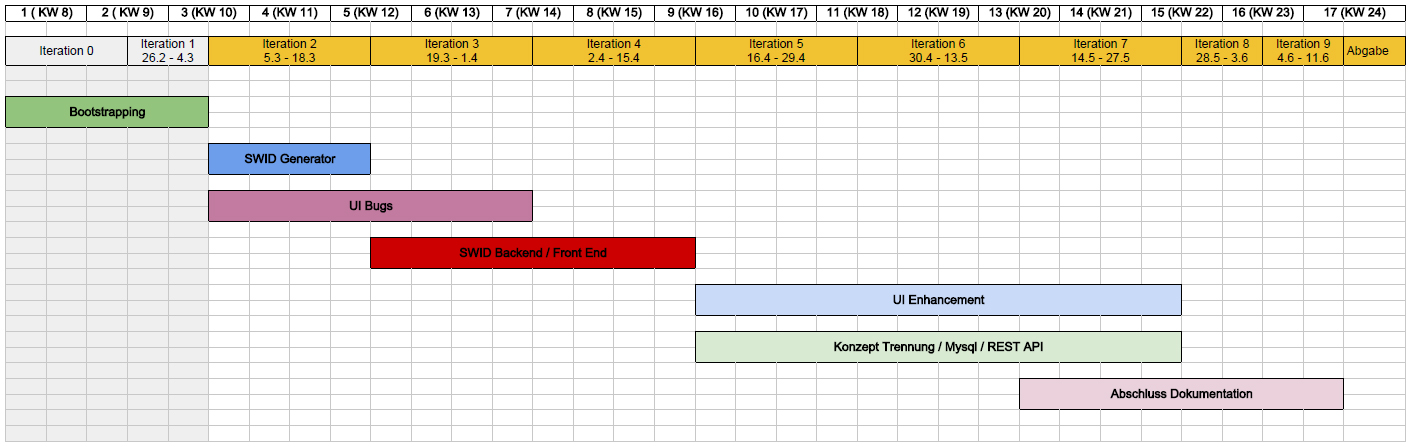
\includegraphics[scale=0.3]{images/zeitplanung/Iteration1_2.jpg}
\subsection{Meeting 3 5.3.2014}
\paragraph{Status}
Eine initiale Planung wurde erstellt. Die Planung ist so ausgelegt, das als erstes die Pflichtteile erarbeitet werden sollen. Einerseits zur Risikominierung für uns und andererseits soll dadruch sichergestellt sein, dass die geforderte Funktionalität,  die Herr Steffen im Juni demonstrieren will, möglichst bald fertig ist und danach ausgiebig getestet werden kann und bis zur Präsentation einen möglichst stabilen Stand erreicht. Sobald diese Funktionalitäten erreicht sind, werden die optionalen Teile in einem separaten Fork integriert um die Stabilität weiterhin zu gewährleisten.
Das SQLite Schema wurde testweise auf MySql/Maria DB portiert. Dabei wurden einige Probleme festgestellt:
\begin{itemize}
\item Tabellennamen sowie Felder verwenden MySql Keywords wie Key/Keys
\item Es gibt Indizes über Felder des Types TEXT, das ist in Mysql so nicht möglich, eine einschränkung über deren länge ist nötig.
\item Die Referenzen in SQLite Syntax sind nur zur dokumentation vorhanden, sind aber leider etwas fehlerhaft. Es gibt verweise auf die nicht existente Tabelle measurements und einige Referenzen fehlen ganz. 
\end{itemize}

\paragraph{Zusammenfassung}

\begin{itemize}
\item Pflichtteile werden in der Planung priorisiert.
\item Die Migration auf MySQL wird nach hinten geschoben, da nicht pflicht und einige Probleme daraus resultieren könnten
\item
\end{itemize}
\subsection{Meeting 4 12.3.2014}
\paragraph{Status}
Der Zeitplan konnte bisher eingehalten werden. Der Stand des SWID Generators konnte im Meeting vorgeführt werden, sieht soweit gut aus. 
Die File Tags sollen optional im output enthalten sein, um das Mapping von Files und Pakete zu erhalten. Dazu gibt es einen Use Case welchen wir im Frontend auch berücksichtigen sollten, siehe Todo. Wir haben noch lange über das Sequenzdiagramm diskutiert, es gibt es da noch einige Zuständigkeiten der einzelnen Komponenten, die noch nicht ganz klar sind. Wir werden das nächste Meeting das überarbeitete Diagramm nochmals mitbringen.

\paragraph{Zusammenfassung}
\begin{itemize}
\item Parameter für xml dokument separator (default: 2x newline)
\item Use gibt einen UseCase: File Hash stimmt nicht, aus welchem Pakage kommt das file?
\item Autodetection des Environments (dpkg/yum)
\item Deployment soll als executable vorliegen, dass zb mittels pip installiert werden kann
\item Nur installierte Packages auflisten, ist momentan noch nicht implementiert
\end{itemize}

\section{Iteration 3}
\subsection{Zeitplanung}
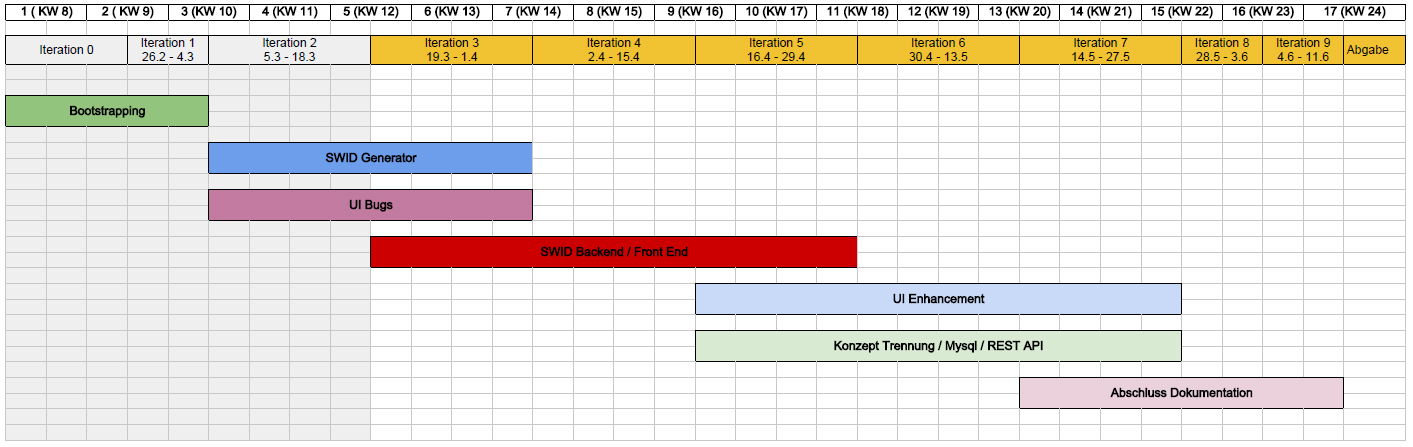
\includegraphics[scale=0.3]{images/zeitplanung/Iteration3.jpg}
\subsection{Meeting 19.3.2014}
\paragraph{Status}

Wir liegen nicht ganz im Zeitplan, da Danilo zur Zeit noch im Spital ist. Entsprechend haben wir den Zeitplan angepasst und die Ziele etwas nach hinten in den vorgesehenen Puffer verschoben. Bis auf das File Listing konnten wir in dieser Iteration alle Ziele erreichen. Wir haben am Meeting eine erste Version des Datenmodells für die SWID Tag vorgestellt. Es gabe da einige Diskussionspunkte. Zum einen stellte sich die Frage ob wir die Daten in das bestehende Modell integrieren sollen oder komplett als Erweiterung (separate Tabellen). Folgende Punkte sind in der Diskussion aufgefallen
\begin{itemize}
\item XML String sollte RAW auch abgespeichert werden

\paragraph{Zusammenfassung}
\begin{itemize}
\item Readme für die SWID Generator Installation erstellen
\item Die Anforderungen ans Backend sind noch nicht sehr klar, wir beginnen mit erfassen von Use Cases, damit könnten sich viele Fragen zum Datenmodell beantworten lassen.
\item Blacklist Option im Package View ist überflüssig
\item Pull Request von aktuellem Stand (strongTNC) erstellen
\item Beim UI sollte bei der Suche bzw. Autocomplete auch die Option angeboten werden ein neues Item zu erstellen -> Usability
\end{itemize}
\end{itemize}



\cleardoublepage % Empty page before the start of the next part

%------------------------------------------------

\ctparttext{TODO Introductory text}

\part{The Library}

%\include{chapters/3}
%\include{chapters/4}
%\include{chapters/5}

%------------------------------------------------

\ctparttext{How was the library developed? What tools were used? What design
decisions were made?}

\part{The Development Process}

%\include{chapters/6}
%\include{chapters/7}

%----------------------------------------------------------------------------------------
%	THESIS CONTENT - APPENDICES
%----------------------------------------------------------------------------------------

\appendix

\part{Appendix} % New part of the thesis for the appendix

%\include{chapters/0A} % Appendix A
%\include{chapters/0B} % Appendix B - empty template

%----------------------------------------------------------------------------------------
%	POST-CONTENT THESIS PAGES
%----------------------------------------------------------------------------------------

\cleardoublepage% Bibliography

\label{app:bibliography} % Reference the bibliography elsewhere with \autoref{app:bibliography}

\manualmark
\markboth{\spacedlowsmallcaps{\bibname}}{\spacedlowsmallcaps{\bibname}} 
\refstepcounter{dummy}

\addtocontents{toc}{\protect\vspace{\beforebibskip}} % Place the bibliography slightly below the rest of the document content in the table of contents
\addcontentsline{toc}{chapter}{\tocEntry{\bibname}}

\bibliographystyle{plainnat}

\bibliography{bibliography}
 % Bibliography

\cleardoublepage% Declaration

\refstepcounter{dummy}
\pdfbookmark[0]{Declaration}{declaration} % Bookmark name visible in a PDF viewer

\chapter*{Declaration} % Declaration section text

\thispagestyle{empty}

Hereby I acknowledge,

\begin{itemize}
		\item that I conducted this thesis by myself and without any external help,
			except with those, which are explicitly mentioned,
		\item that all used sources are cited academically correct, and 
		\item that I didn't use any copyright protected materials (e.g. images) in
			an unauthorized manner.
\end{itemize}

\bigskip
 
\noindent\textit{\myLocation, \myTime}

\bigskip

\begin{flushright}
\begin{tabular}{m{8cm}}
\hspace{2cm}
\includegraphics[width=.33\textwidth]{images/signature.png}
\\ \hline
\centering\myName, \today \\
\end{tabular}
\end{flushright}
 % Declaration

%----------------------------------------------------------------------------------------

\end{document}
